\section{Szyfrowanie}

\begin{frame}
	\begin{alertblock}{Szyfrowanie}
			Jest to proces przetwarzania przesyłanej informacji w taki sposób, by była czytelna tylko dla uprawnionych stron komunikacji. Wiadomość zostaje przesłana w zakodowanej postaci, co znacznie utrudnia lub uniemożliwia zrozumienie jej treści w przypadku przechwycenia.
	\end{alertblock}
\end{frame}

\begin{frame}{Szyfrowanie symetryczne}
	Zarówno odbiorca, jak i nadawca dysponują takim samym kluczem.\\
	\vspace{\fill}
	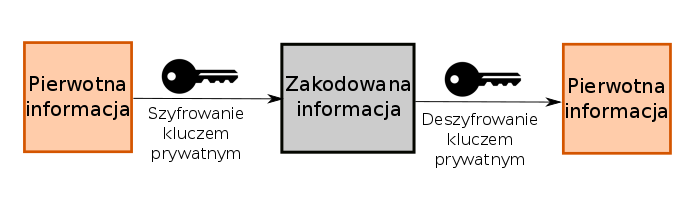
\includegraphics[height=0.25\paperwidth]{images/priv-key.png}
	\vspace{\fill}
	Obie strony muszą znać klucz przed rozpoczęciem komunikacji. Zwiększa to prawdopodobieństwo jego przechwycenia.	
\end{frame}

\begin{frame}{Szyfrowanie asymetryczne}
		\begin{itemize}
			\item Generowane są dwa klucze, prywatny i publiczny.
			\item Klucz publiczny jest ogólnie dostępny.
			\item Utworzenie dwóch takich par eliminuje konieczność wymiany kluczów prywatnych. 
		\end{itemize}	
\end{frame}

\begin{frame}{Szyfrowanie asymetryczne}
		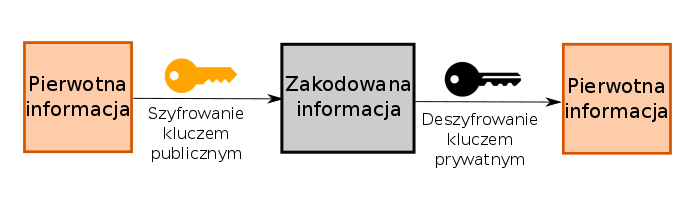
\includegraphics[height=0.25\paperwidth]{images/pub-key.png} \\
		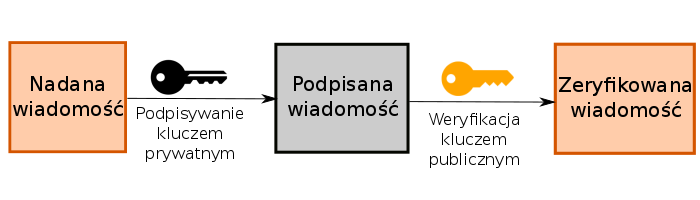
\includegraphics[height=0.25\paperwidth]{images/pub-key-sign.png}
\end{frame}

\begin{frame}{Algorytmy szyfrujące asymetrycznie}
	\begin{itemize}
		\item Digital Signature Algorithm (DSA).
		\item ElGamal.
		\item NTRUEncrypt.
		\item Algorytmy bazujące na kryptografii krzywych eliptycznych.
		\item RSA.
	\end{itemize}
\end{frame}

\begin{frame}{Algorytmy szyfrujące symetrycznie}
	\begin{itemize}
		\item Advanced Encryption Standard (AES).
		\item Data Encryption Standard (DES).
		\item Blowfish.
		\item IDEA.
		\item RC4.
		\item Tiny Encryption Algorithm.
	\end{itemize}
\end{frame}

\begin{frame}{Symetryczne --- po co?}
	\begin{itemize}
		\item Algorytmy symetryczne są dużo tańsze i prostsze obliczeniowo (mniejsze obciążenie CPU, tańsze koszty utrzymania serwerów, znacząco szybsze prędkości zapisu na szyfrowane nośniki itd.).
		\item AES ma nawet swoje natywne instrukcje w niektórych CPU.
		\item Pozostaje problem bezpiecznej wymiany klucza prywatnego.
		\item Rozwiązaniem jest wymiana klucza w \emph{asymetrycznie} szyfrowanym kanale i dopiero późniejsze przejście na komunikację \emph{symetryczną}.
	\end{itemize}
\end{frame}

\subsection{Protokoły}

\begin{frame}{Protokoły}
	W celu zagwarantowania bezpieczeństwa transmisji danych w sieci, w ustandaryzowanym pakiecie protokołów internetowych wykorzystane szereg metod kryptograficznych.
	\begin{center}
		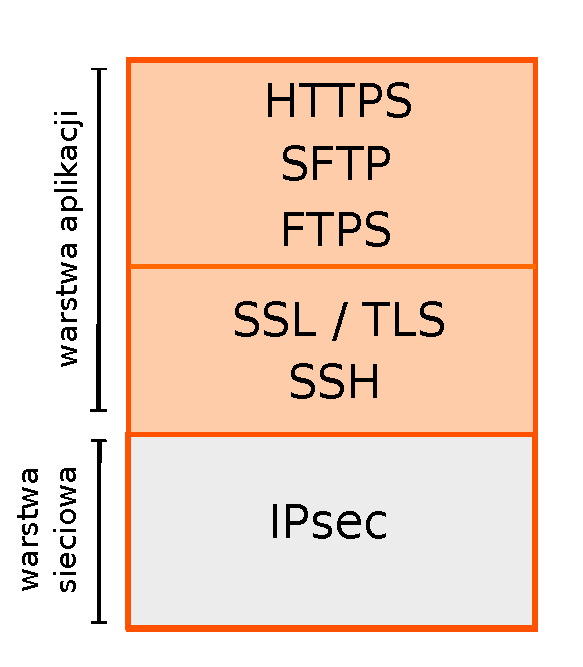
\includegraphics[height=0.4\paperwidth]{images/protocols.pdf}	
	\end{center}

\end{frame}

\begin{frame}{IPsec}
	\begin{alertblock}{Internet Protocol Security}
		Zestaw protokołów wykorzystujących szyfrowanie pakietów i uwierzytelnianie na poziomie warsty sieciowej. 
	\end{alertblock}
		\vspace{\fill}
		Może zostać zaimplementowany w dwóch trybach:
		
		\begin{enumerate}
			\item \textbf{transportowym} — szyfrowane są tylko dane;
			\item \textbf{tunelowym} — szyfrowany jest cały pakiet.
		\end{enumerate}
\end{frame}

\begin{frame}{SSH}
	\begin{alertblock}{Secure Shell}
		Protokół wykorzystujący kryptografię asymetryczną do bezpiecznego zdalnego dostępu do komputera. 
	\end{alertblock}
	
	Połączenie jest realizowane w architekturze klient--serwer. Uwierzytelnienie może zostać przeprowadzone w dwóch wariantach:
	\begin{enumerate}
		\item z automatycznym generowaniem par kluczy oraz wykorzystaniem hasła (tzw. wariant BZP --- bardzo złego pomysłu);
		\item z ręcznym generowaniem kluczy.
	\end{enumerate}
	
\end{frame}

\begin{frame}{SSH}
	Protokół SSH charakteryzuje się szerokim spektrum zastosowań:
	\begin{itemize}
		\item zdalne wykonywanie komend (które mogą być organiczone na serwerze, a nawet dowolnie przez niego interpretowane, por. \href{https://medium.com/@shazow/ssh-how-does-it-even-9e43586e4ffc}{chat over SSH}, \href{http://gitolite.com/}{Gitolite} itd.);
		\item tunelowanie/przekierowywanie portów TCP;
		\item przekazywanie sesji graficznej X11 (system okien);
		\item przesył plików.
	\end{itemize}
\end{frame}

\begin{frame}{TLS}
	\begin{alertblock}{Transport Layer Security}
		Protokół zapewniający bezpieczną wymianę informacji pomiędzy aplikacjami w obrębie Internetu. W celu uwierzytelnienia stron wykorzystuje certyfikację.
	\end{alertblock}
\end{frame}

\begin{frame}{TLS}
	TLS również bazuje na architekturze klient-serwer. Można wyróżnić dwie warstwy komunikacji:
	\vspace{\fill}
	\begin{enumerate}
		\item \textbf{„uścisk dłoni”} — komunikacja szyfrowana asymetrycznie — w tej fazie dochodzi do uwierzytelnienia stron oraz negocjacji formatowania i porządku wymiany wiadomości oraz klucza prywatnego używanego w 2 etapie;
		\vspace{\fill}
		\item \textbf{wymiana danych} — szyfrowanie symetryczne — wiadomości przechodzą proces kapsułkowania, tworząc zaszyfrowane rekordy, których spójność jest weryfikowana.
	\end{enumerate}
\end{frame}

\begin{frame}{SSL vs TLS}
	Protokół SSL jest obecnie uznawany jako przestarzały poprzednik TLS. Względem SSL dodano następujące usprawnienia:
	\begin{itemize}
		\item bezpieczniejsze funkcje haszujące;
		\item wyrugowano błędy logiczne;
		\item standaryzacja w RFC 2246;
		\item rozluźniono restrykcje przy pozyskiwaniu certyfikatów z urzędów uwierzytelniających;
		\item dodatkowe wiadomości z ostrzeżeniami.
	\end{itemize} 
\end{frame}

\begin{frame}{Warstwy protokołów}
	\begin{table}
	\centering
		\begin{tabular}{| l | c | r |}
			\hline
			\parbox[t]{1in}{
			Protokół
			\par kryptograficzny} & \parbox[t]{1in}{Protokół 
			\par bez szyfrowania} & \parbox[t]{1in}{Warstwa \par wynikowa} \\		
			\hhline{|=|=|=|} 
			\multirow{2}{*}{TLS} & HTTP & HTTPS \\ 
			& FTP & FTPS \\                 
			\hline
			\multirow{2}{*}{SSH} & FTP & SFTP \\ 
			& RCP & SCP \\                 
			\hline    
		\end{tabular}
	\end{table}	
\end{frame}

